

\subsubsection{Estimation of the Discount Rate Ke.}

The higher the systematic risk of a stock, the higher the return that investors will expect from equity securities. In order to estimate an appropriate discount rate in nominal terms and after taxes, the following inputs were used to determine the value of the \textcolor{principal}{Weighted Average Cost of Capital (WACC):}\\

\textcolor{principal}{Risk-free rate (Rf).} It is based on the yield of government bonds; in this case, the yield of the Mexican 10-year bond was considered, according to the website \url{Tradingeconomics.com}, with the following result:\\

\begin{figure}[H]
\centering
The risk-free rate obtained is \textbf{\rfValor\%}.\\[5pt]

\caption{Mexican  10-Year Bond Interest Rate Expectations}
 \includegraphics[width=9cm]{../0.imagenes_eng/rf}
\end{figure}


\gls{beta}. In order to determine the appropriate Beta ($\beta$) factor for the business, a market sample of levered betas from companies comparable to the valued business was considered:\\


\begin{figure}[H]
\centering
\includegraphics[width=.9\textwidth]{../0.imagenes_eng/beta_1}\\
\end{figure}

The levered beta of the sector corresponding to the company is \textcolor{principal}{\textbf{\valorBeta x}} (mean).\\

Unlevered Beta Formula:\\

\begin{figure}[H]
\centering

\includegraphics[width=8cm]{\rutaImagenes/beta_apalancada}
\end{figure}


The appraiser conducted the estimation of the unlevered BETA forecast for the business, having applied to the debt/equity ratio of the subject, the sample average, and the effective tax rate of the sector (ETR); with a result of \textcolor{principal}{\betaDesapalancada x}.\\

Relevered Beta Formula:\\

\begin{figure}[H]
\centering

\includegraphics[width=8cm]{\rutaImagenes/beta_reapalancada}
\end{figure}

Once the sector's unlevered BETA indicator was obtained, the appraiser carried out the estimation of the forecast for the relevered BETA to the business subject to valuation, having applied to the debt/equity ratio of the subject, the sector sample's median, and the Marginal tax rate of Mexico (MTR), with a result of  \textcolor{principal}{\betaReapalancada x}.\\

\textcolor{principal}{Equity Market Risk Premium:} It was obtained from the historical average of the difference in returns or ``spread'' between the Mexican stock market using the indicator known as the   enterprise risk premium (ERP).\\

\begin{figure}[H]
\centering
The enterprise risk premium is \textbf{\textcolor{principal}{\erpValor\%}} \\[10pt]

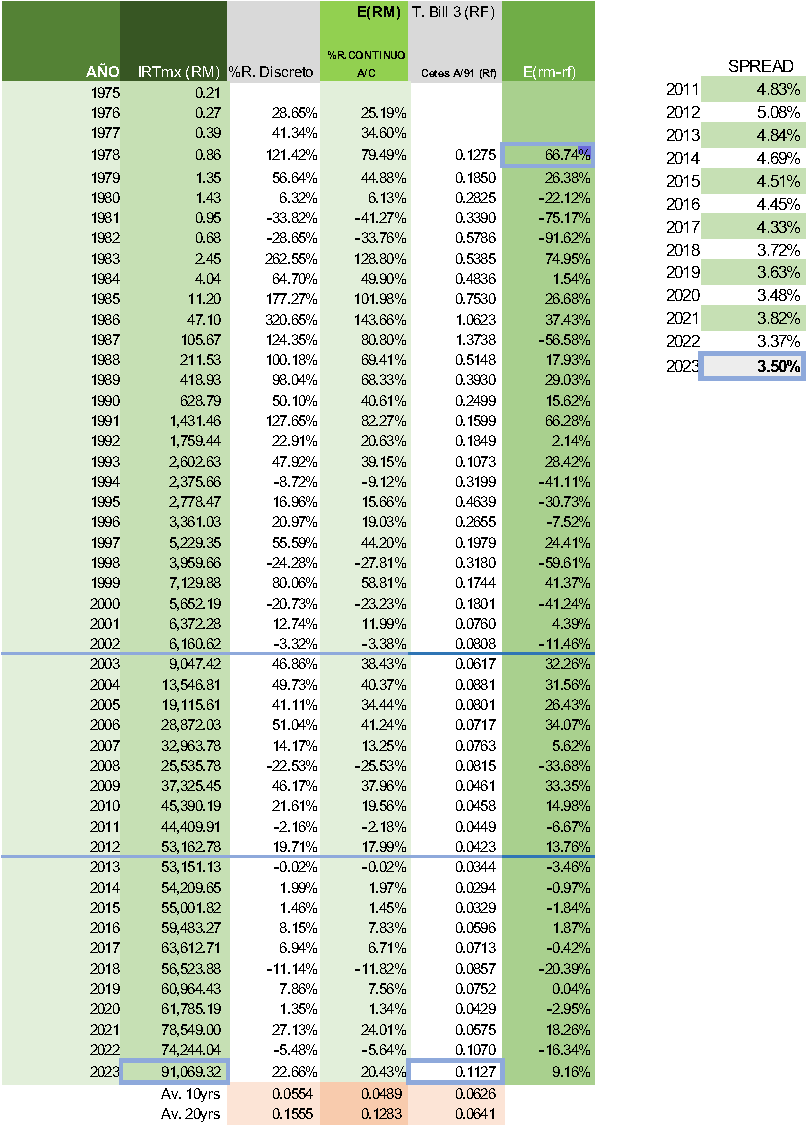
\includegraphics[width=.6\textwidth]{../0.imagenes_eng/erp}
\end{figure}

%\newpage
\textcolor{principal}{\textit{Size Prime}.} \\[5pt]

A size premium was applied to the firm, based on the book value of equity according to the following table.\\


\begin{figure}[H]
\centering
The Size Prime is \textbf{\textcolor{principal}{\sizePrime\%}} \\
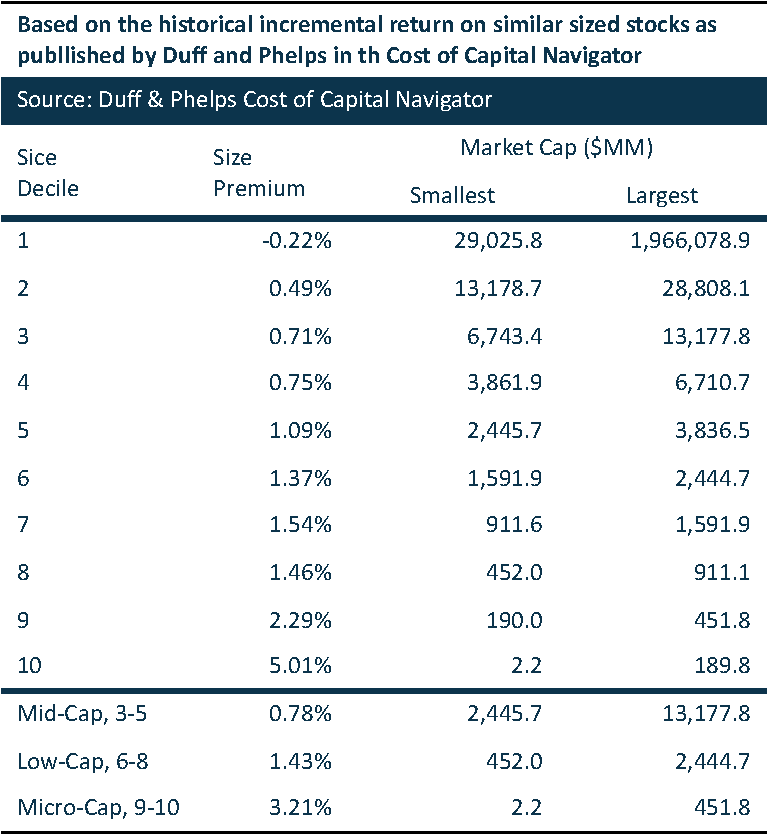
\includegraphics[width=.5\textwidth]{\rutaImagenes/sp}
\end{figure}


Estimation of the Cost of Equity (Ke), resulting in \textcolor{principal}{\keValor\%}, 
in accordance with observable rates in the Mexican market:

\begin{figure}[H]
\centering
\includegraphics[width=10cm]{../0.imagenes_eng/ke}
\end{figure}








